\documentclass[a4paper, 12pt]{article}%тип документа

%%%Библиотеки
	%\usepackage[warn]{mathtext}	
	\usepackage[T2A]{fontenc} % кодировка
	\usepackage[utf8]{inputenc} % кодировка исходного текста
	\usepackage[english,russian]{babel} % локализация и переносы
	\usepackage{caption}
	\usepackage{listings}
	\usepackage{amsmath,amsfonts,amssymb,amsthm,mathtools}
	\usepackage{wasysym}
	\usepackage{graphicx}%Вставка картинок правильная
	\usepackage{float}%"Плавающие" картинки
	\usepackage{wrapfig}%Обтекание фигур (таблиц, картинок и прочего)
	\usepackage{fancyhdr} %загрузим пакет
	\usepackage{lscape}
	\usepackage{xcolor}
	\usepackage[normalem]{ulem}
	\usepackage{hyperref}

%%%Конец библиотек




%%%Настройка ссылок
	\hypersetup
	{
		colorlinks=true,
		linkcolor=blue,
		filecolor=magenta,
		urlcolor=blue
	}
%%%Конец настройки ссылок


%%%Настройка колонтитулы
	\pagestyle{fancy}
	\fancyhead{}
	\fancyhead[L]{Лабораторная работа}
	\fancyhead[R]{Талашкевич Даниил, группа Б01-009}
	\fancyfoot[C]{\thepage}
%%%конец настройки колонтитулы



							\begin{document}
						%%%%Начало документа%%%%


%%%Начало титульника
\begin{titlepage}

	\newpage
	\begin{center}
		\normalsize Московский физико-технический институт \\(госудраственный 			университет)
	\end{center}

	\vspace{6em}

	\begin{center}
		\Large Лабораторная работа по оптике\\
	\end{center}

	\vspace{1em}

	\begin{center}
		\large \textbf{Кольца Ньютона [4.2.1]}
	\end{center}

	\vspace{2em}

	\begin{center}
		\large Талашкевич Даниил Александрович\\
		Группа Б01-009
	\end{center}

	\vspace{\fill}

	\begin{center}
	Долгопрудный \\2022
	\end{center}
	
\end{titlepage}
%%%Конец Титульника



%%%Настройка оглавления и нумерации страниц
	\thispagestyle{empty}
	\newpage
	\tableofcontents
	\newpage
	\setcounter{page}{1}
%%%Настройка оглавления и нумерации страниц


					%%%%%%Начало работы с текстом%%%%%%

\section{Аннотация}

$\text{ }$

$\textbf{Цель работы}$ : ознакомление с явлением интерференции в тонких пленках (полосы равной толщины) на примере колец Ньютона и с методикой интерференционных измерений кривизны стеклянной поверхности.

$\textbf{В работе используются}$ : измерительный микроскоп с опак-иллюминатором; плосковыпуклая линза; пластинка из черного стекла; ртутная лампа ПРК-4; щель; линзы; призма прямого зрения; объектная пікала.

\section{Теоретические сведения}

Интерференция -- взаимное увеличение или уменьшение результирующей амплитуды двух или нескольких когерентных волн при их наложении друг на друга.

Кольца Ньютона -- кольцеобразные интерференционные максимумы и минимумы, появляющиеся вокруг точки касания слегка изогнутой выпуклой линзы и плоскопараллельной пластины при прохождении света сквозь линзу и пластину.

В нашей установке кольца Ньютона образуются при интерференции световых волн, отраженных от границ тонкой воздушной прослойки, заключенной между выпуклой поверхностью линзы и плоской стеклянной пластинкой (рис. 1). Наблюдение ведется в отраженном свете.

\begin{figure}[!h]
\label{1}
\begin{center}
	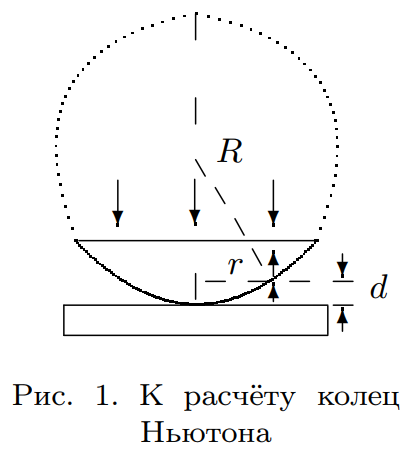
\includegraphics[scale=0.5]{1.png}
\end{center}
\end{figure}

Этот классический опыт используется для определения радиуса кривизны сферических поверхностей линз. В этом опыте наблюдается интерференция волн, отражённых от границ тонкой воздушной прослойки, образованной сферической поверхностью линзы и плоской стеклянной пластиной. При нормальном падении света (рис. 1) интерференционные полосы локализованы на сферической поверхности и являются полосами равной толщины.
	
	Геометрическая разность хода между интерферирующими лучами равна удвоенной толщине воздушного зазора $ 2d $ в данном месте. Для точки на сферической поверхности, находящейся на расстоянии $ r $ от оси системы, имеем $ r^2 = R^2 - (R - d)^2 = 2Rd - d^2 $, где $ R $ -- радиус кривизны сферической поверхности (рис. \ref{1}).
	
	При $ R \gg d $ получим $d = r^2/2R $. С учётом изменения фазы на $ \pi $ при отражении волны от оптически более плотной среды (на границе воздух-стекло) получим \textbf{оптическую разность хода интерферирующих лучей}:
	
	\begin{equation}\label{r_m}
	\Delta = \dfrac{\lambda}{2} + 2d = \dfrac{r^2}{2R} + \dfrac{\lambda}{2}
	\end{equation}
	
	Из условия интерференционного минимума $ \Delta = \dfrac{(2m +1)\lambda}{2}, \; m =0, 1, 2, \dots $ . Получим радиусы темных колец $ r_m $, а из аналогичного условия максимума $ \Delta = m \lambda $ радиусы светлых $ r_m' $ :
	
	\begin{equation}\label{r_m'}
	r_m = \sqrt{m \lambda R}, \qquad 	r_m' = \sqrt{\dfrac{(2m-1)m \lambda R}{2}}
	\end{equation}


\section{Экспериментальная установка}

Схема экспериментальной установки приведена на рис. \ref{lab}. Опыт выполняется с помощью измерительного микроскопа.
На столик микроскопа помещается держатель с полированной пластинкой из
чёрного стекла. На пластинке лежит исследуемая линза.

	\begin{figure}[!h]
	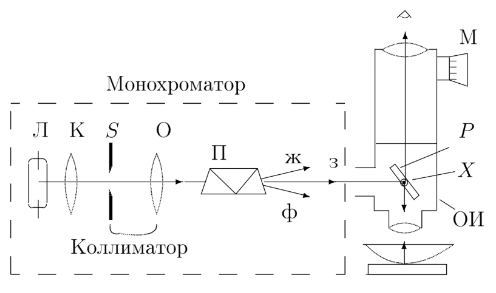
\includegraphics[width=\linewidth]{2.png}
	\caption{Экспериментальная установка}
	\label{2}
	\end{figure}

	Источником света служит ртутная лампа, находящаяся в защитном кожухе. Для получения монохроматического света применяется призменный монохроматор, состоящий из конденсора $ К $, коллиматора (щель $ S $ и объектив $ О $) и призмы прямого зрения $ П $. Эти устройства с помощью рейтеров располагаются на оптической скамье. Свет от монохроматора попадает на расположенный между объективом и окуляром микроскопа опак-иллюминатор (ОИ)  специальное устройство, служащее для освещения объекта при работе в отражённом свете. Внутри опак-иллюминатора находится полупрозрачная стеклянная пластинка P, наклоненная под углом $ 45^\circ $ к оптической оси микроскопа. Свет частично отражается от этой пластинки, проходит через объектив микроскопа и попадает на исследуемый объект. Пластинка может поворачиваться вокруг горизонтальной оси $ X $, опак-иллюминатор вокруг вертикальной оси.

	Столик микроскопа может перемещаться в двух взаимно перпендикулярных направлениях помощью винтов препаратоводителя. Отсчетный крест окулярной шкалы перемещается перпендикулярно оптической оси с помощью микрометрического винта $ М $.
	
	Оптическая схема монохроматора позволяет получить в плоскости входного окна опак-иллюминатора достаточно хорошо разделённые линии спектра ртутной лампы. Изображение щели $ S $ фокусируется на поверхность линзы объективом микроскопа, т.е. точка источника и точка наблюдения спектра совпадают.Интерференционная картина не зависит от показателя преломления линзы и определяется величиной зазора между линзой и пластинкой (кольца равной толщины).

	Сначала микроскоп настраивается на кольца Ньютона в белом свете (свете ртутной лампы), затем при помощи монохроматора выделить из спектра яркую зелёную линию и провести измерения диаметров колец в монохроматическом свете. 
	

\section{Ход работы}

\section{Обработка данных}

\section{Вывод}

 
\section{Литература}

\begin{enumerate}

\item .

\end{enumerate}	

\end{document}
